\documentclass[12pt,a4paper]{article}
\usepackage{verbatim}
\usepackage{graphicx}
\usepackage{amsmath}
\usepackage{float}
\author{ZHANG Xiao Research Intern in IBM CRL}
\title{Network 20q HW8}

\begin{document}
\maketitle
\pagebreak

\section{TCP slow start}
In this question, while the windows size of a TCP session $w$ would increase by 1 for each ACK received. So for a connection without lost, we would have the following transition.


\begin{equation}
\begin{tabular}{ l l l l }
\hline
Round & Add-on & Current Window Size \\
\hline
 1 & 0 & 1 \\
 2 & 1 & 2 \\
 3 & 2 & 4 \\
 4 & 4 & 8 \\
 $\cdots$ &  $\cdots$ &  $\cdots$ \\
 n  & $2^{n-2}$ &  $2^{n-1}$ \\
\hline
\end{tabular}
\end{equation}

The Window Size would grow exponentially with the time slide.

So the time-space diagram for the first four RTT would be like:

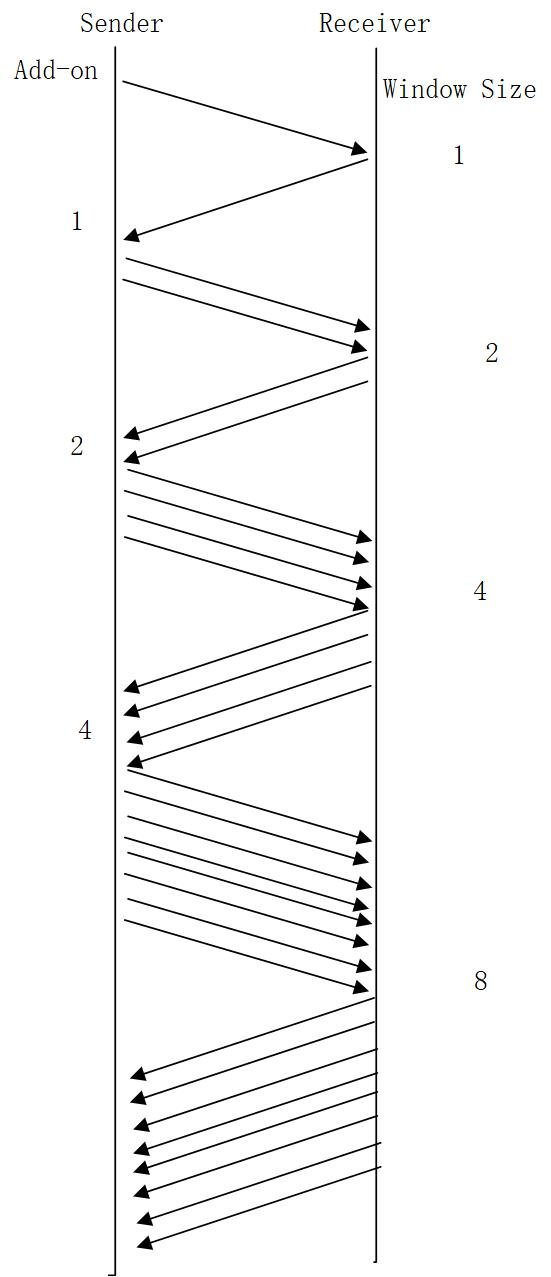
\includegraphics{PIC/network.png}

\section{Embedding Tree}

\subsection{a}

\begin{equation}
r_{max} = min\{u_s, \frac{u_s+\sum{u_i}}{N}\} = min\{2, \frac{2+3+2+1}{3}\} = min\{2,\frac{8}{3}\} = 2
\end{equation}

All the 2-hop tree would satisfy this condition:

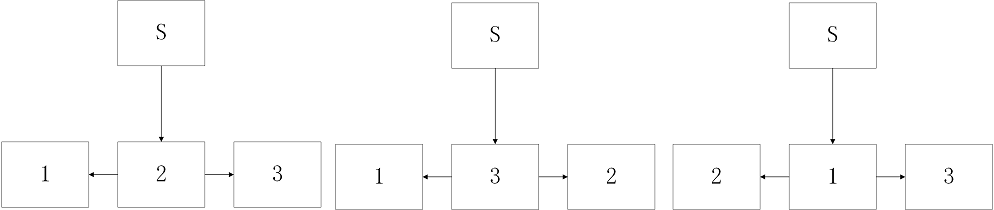
\includegraphics{PIC/embed-tree-a.png}

\subsection{b}
\begin{equation}
r_1 = \frac{2}{1+2+3} * 2 = \frac{2}{3}
\end{equation}
\begin{equation}
r_1 = \frac{1}{1+2+3} * 2 = \frac{1}{3}
\end{equation}
\begin{equation}
r_1 = \frac{3}{1+2+3} * 2 = 1
\end{equation}

\subsection{c}

Under this condition, the link could only pass one link, so the graph would be like the following, and the speed would be the lowest speed.

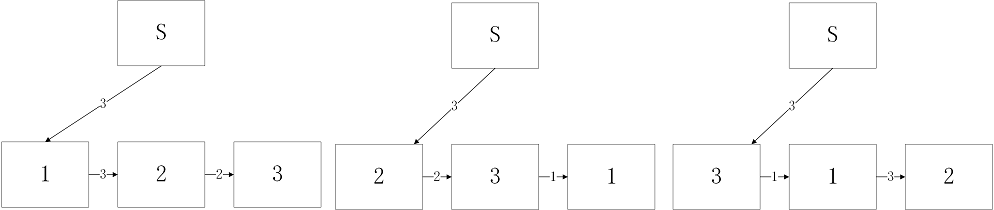
\includegraphics{PIC/embed-tree-c.png}

\begin{equation}
r_1 = 2
\end{equation}
\begin{equation}
r_2 = 1
\end{equation}
\begin{equation}
r_3 = 1
\end{equation}


\end{document}